\documentclass[12pt]{ociamthesis}  % default square logo 
%\documentclass[12pt,beltcrest]{ociamthesis} % use old belt crest logo
%\documentclass[12pt,shieldcrest]{ociamthesis} % use older shield crest logo

%load any additional packages
\usepackage{amssymb}
\usepackage{multirow}

%input macros (i.e. write your own macros file called mymacros.tex 
%and uncomment the next line)
%\include{mymacros}

\title{\large LAPORAN ORACLE APEX  \\[3ex]     %your thesis title,
        \textit{} }   %note \\[1ex] is a line break in the title

\author{Nabilla}             %your name
\college{1184075 \\[5ex]
\textit{}} %your college

%\renewcommand{\submittedtext}{change the default text here if needed}
\degree{Politeknik Pos Indonesia}     %the degree
\degreedate{Bandung}         %the degree date
\degreedate{2019}  

%end the preamble and start the document
\begin{document}

%this baselineskip gives sufficient line spacing for an examiner to easily
%markup the thesis with comments
\baselineskip=18pt plus1pt

%set the number of sectioning levels that get number and appear in the contents
\setcounter{secnumdepth}{3}
\setcounter{tocdepth}{3}


\maketitle                  % create a title page from the preamble info
\begin{dedication}

”Pendidikan adalah paspor untuk masa,untuk hari esok yang dimiliki oleh orang yang mempersiapkan hari ini. \\
(Malcolm X) \\
Barangsiapa tidak mau merasakan pahitnya belajar, ia akan merasakan hinanya kebodohan sepanjang hidupnya, \\ 
(imam Syafi'i rahimahullah) \\

\end{dedication}        % include a dedication.tex file
\begin{acknowledgements}
\par
Assalamualaikum warahmatullahi wabarakatuh. Segala puji bagi Allah SWT yang telah melimpahkan rahmat dan hidayah-Nya, sehingga kami dapat menyelesaikan laporan dengan judul “Laporan Pembelajaran Oracle Academy Virtual Students Day”. Penyusunan laporan ini dimaksudkan untuk memenuhi tugas D4 teknik informatika pada bidang mata kuliah Database II. Dalam penyusunan laporan ini, kami mengucapkan kepada pihak yang telah membantu atau membimbing kami dalam penyusunan laporan ini ini. Laporan ini juga tidak terlepas dari bapak Syafrial Fachri Pane, S.T., M.T.I selaku dosen matakuliah database. Penulis telah membuat laporan ini dengan sebaik-baiknya, diharapkan memberikan kritik dan saran dari semua pihak yang bersifat membangun, terimakasih.

\begin{raggedleft}




\vspace{12ex}
Bandung, 17 Oktober 2019

\vspace{6ex}
Penulis

\end{raggedleft}

\end{acknowledgements}   % include an acknowledgements.tex file
\begin{abstract}
	Panduan Penulisan Jurnal Ilmiah (PPJI) ini dibuat dengan tujuan memberikan acuan bagi para sivitas akademika
	yang memulai menulis jurnal ilmiah. Pada intinya PPJI menjelaskan secara lengkap tentang standar pengerjaan jurnal internasional dari pengalaman penulisan dari tahun 2017. Di dalamnya memuat aturan standar penulisan dan penggunaan Latex sebagai editor. Dengan demikian diharapkan semua sivitas akademika dapat membuat jurnal ilmiah dengan
	 lancar dan sesuai dengan standar.
\end{abstract}          % include the abstract
\begin{abstract}



\textbf{}
\end{abstract}

\begin{romanpages}          % start roman page numbering
\tableofcontents            % generate and include a table of contents
\listoffigures
\listoftables           % generate and include a list of figures
\end{romanpages}            % end roman page numbering

%now include the files of latex for each of the chapters etc
\chapter{Oracle Aplication Express}


\section{Pengertian Oracle APEX}
Oracle Aplication Express\cite{OracleApex}. Adalah sebuah wadah dan sarana untuk membuat aplikasi yang menggunakan database Oracle Itu sendiri, pada kelas Online pertama saya belajar banyak hal cara Menggunakan Aplikasi Oracle Apex online yang di dalam video sudah diberikan link diantaranya Request Workspace, Create Workspace, Membuat Spreadsheet Pertama.

\section{Cara Membuat Aplikasi Sederhana di Apex Oracle Online}
Langkah - langkahnya adalah sebagai berikut :
\begin{enumerate}
    \item Melakukan registrasi untuk masuk pada apex . di tampilan ini user memasukkan nama workspace yang telah dibuat serta memasukkan username dan password. ketika user belum mempunyai workspace . maka user mengklik request a workspace untuk membuat workspace baru .
\newline
    \item   Lalu request a workspace dengan mengisikan first name, last name
    , email dan membuat workspace . kemudian klik next 
\newline
    \item   verifikasi memlalui email . buka email lalu klik pesan dari oracle kemudian klik clik create workspace .
\newline
    \item   Masukkan oracle application express dengan memasukkan nama workspace , masukkan nama user dan password lalu klik sign in
\newline
    \item  Akan keluar tampilan seperti gambar yang sudah terlampir pada platform
    \newline
    \begin{figure} [!htbp]
        \centering
        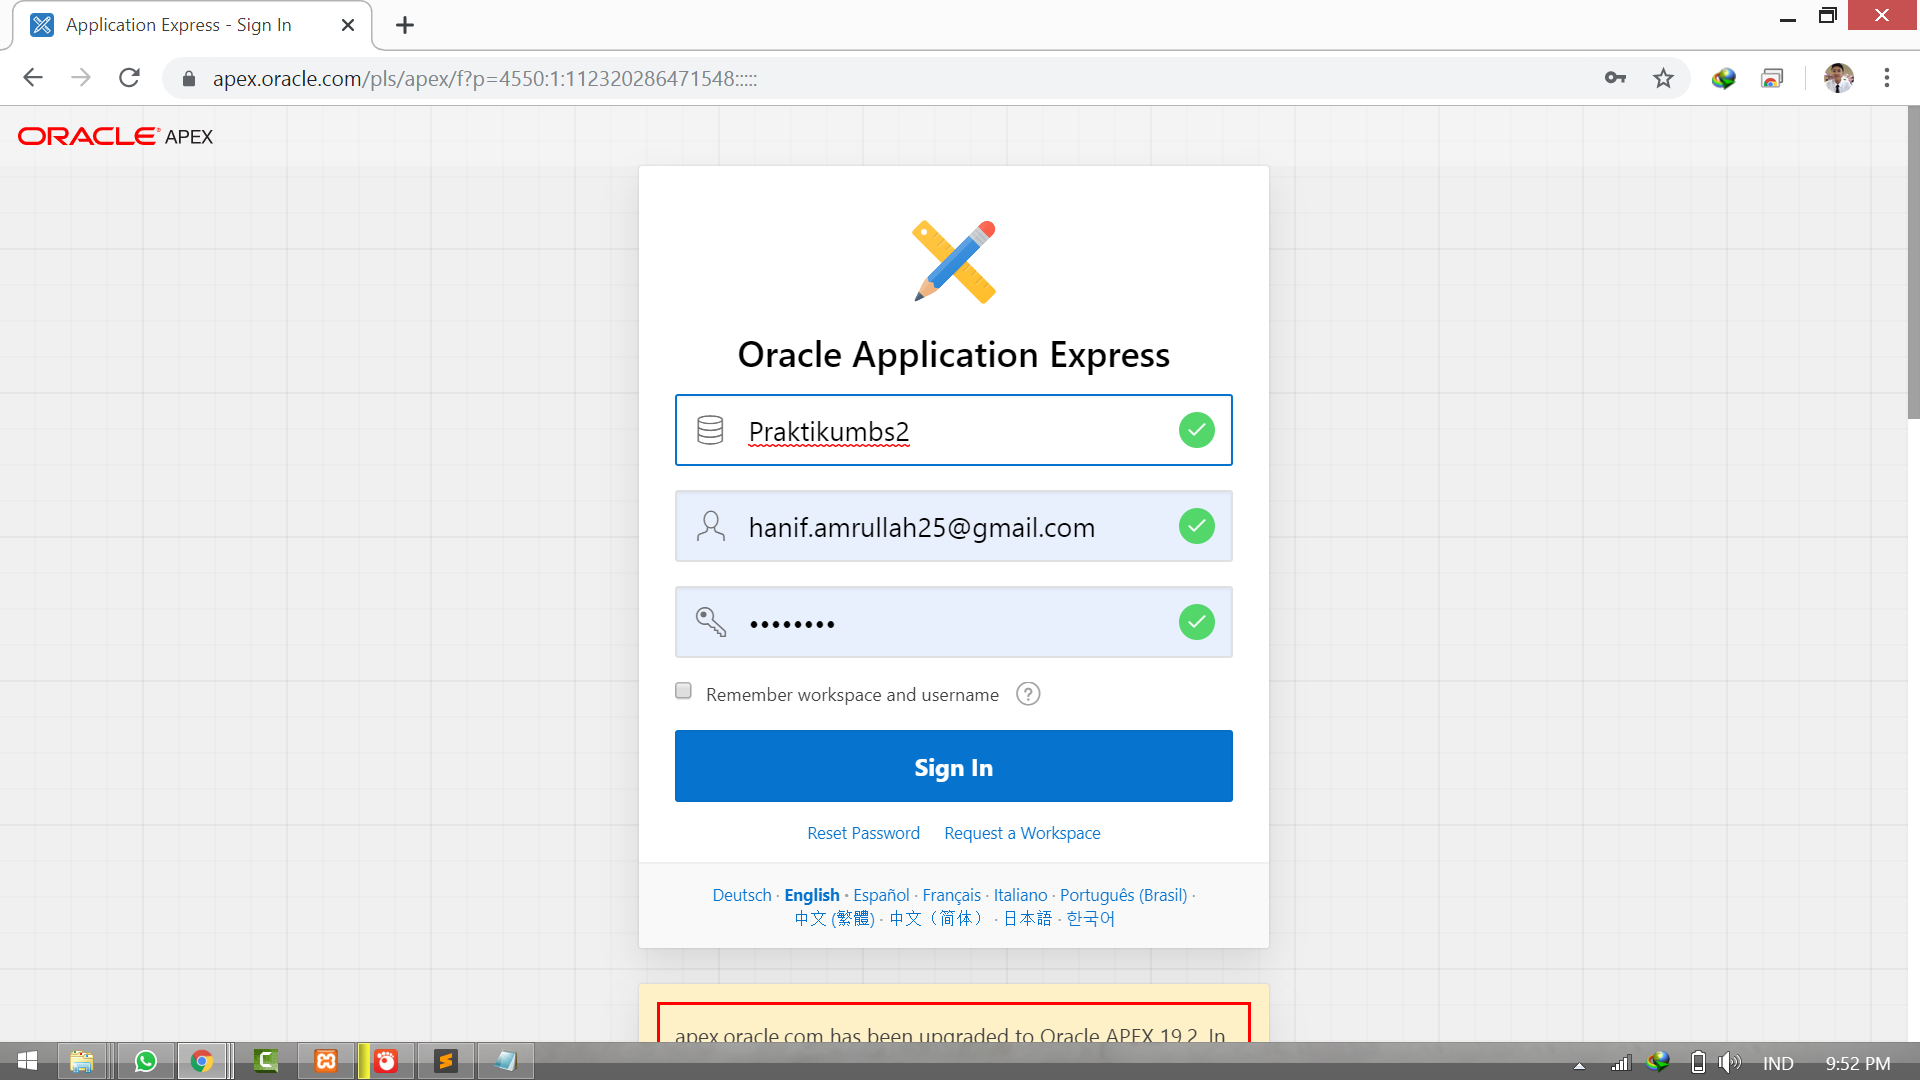
\includegraphics[scale=0.5]{figures/1.png}
        \caption{Create}
        \label{penanda}
    \end{figure}
\newline
    \item  lalu create
\newline
    \item  Setelah itu unggah file dalam bentuk csv,xlxs,xml atau json .
    \newline
    \begin{figure}[!htbp]
        \centering
        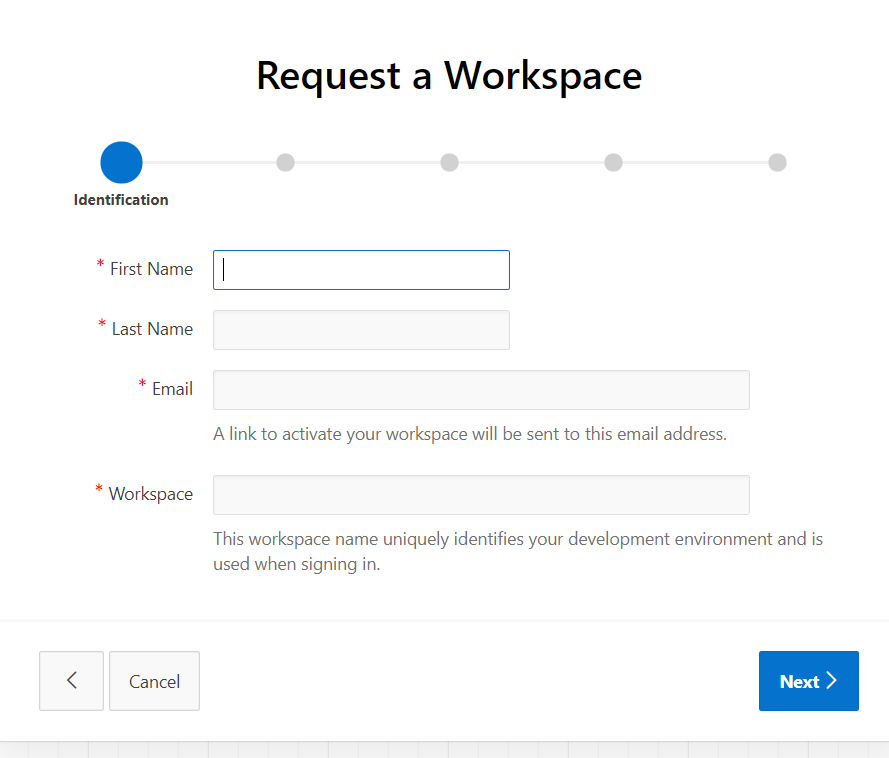
\includegraphics[scale=0.5]{figures/3.png}
        \caption{Memasukan file}
        \label{penanda}
    \end{figure}
\newline
    \item  Kemudian pilih file data excel yang telah dibuat dalam bentuk xlsx
\newline
    \item  Buat tabel dengan memasukkan nama tabel disini saya membuat tabel Mahasiswa terlebih dahulu .
    \newline
    \begin{figure}[!htbp]
        \centering
        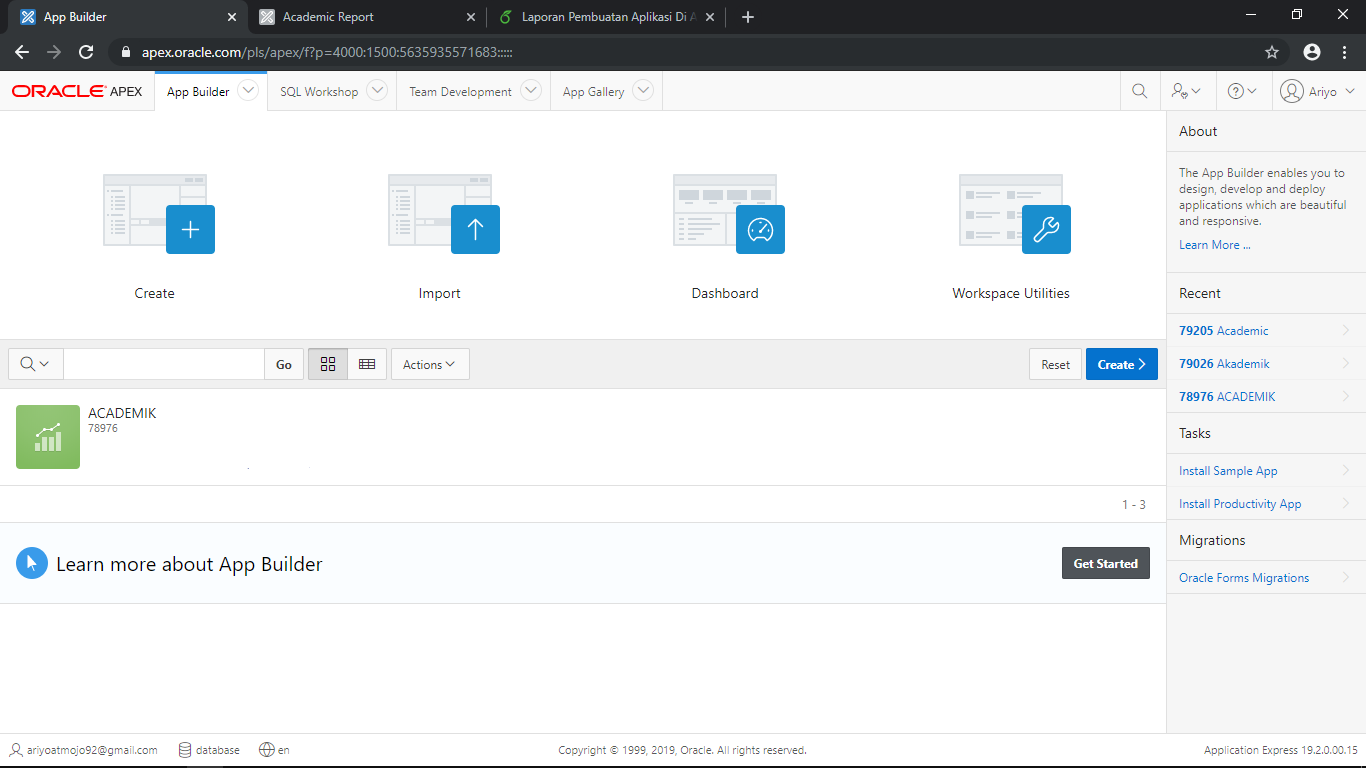
\includegraphics[scale=0.5]{figures/4.png}
        \caption{Membuat nama tabel Mahasiswa}
        \label{fig:my_label}
    \end{figure}
\newline
    \item Klik configure untuk mengecek apakah tabel dari data excel sudah benar atau tidak 
\newline
    \item  Lalu scroll kebawah sehingga keluar daftar nama mahasiswa yang berada pada file excel kemudian klik load data 
\newline
    \item Kemudia klik X untuk membuat tabel berikutnya , lakukan seperti perintah yang diatas lagi . selanjutnya membuat tabel dosen 
\newline
    \begin{figure}[!htbp]
        \centering
        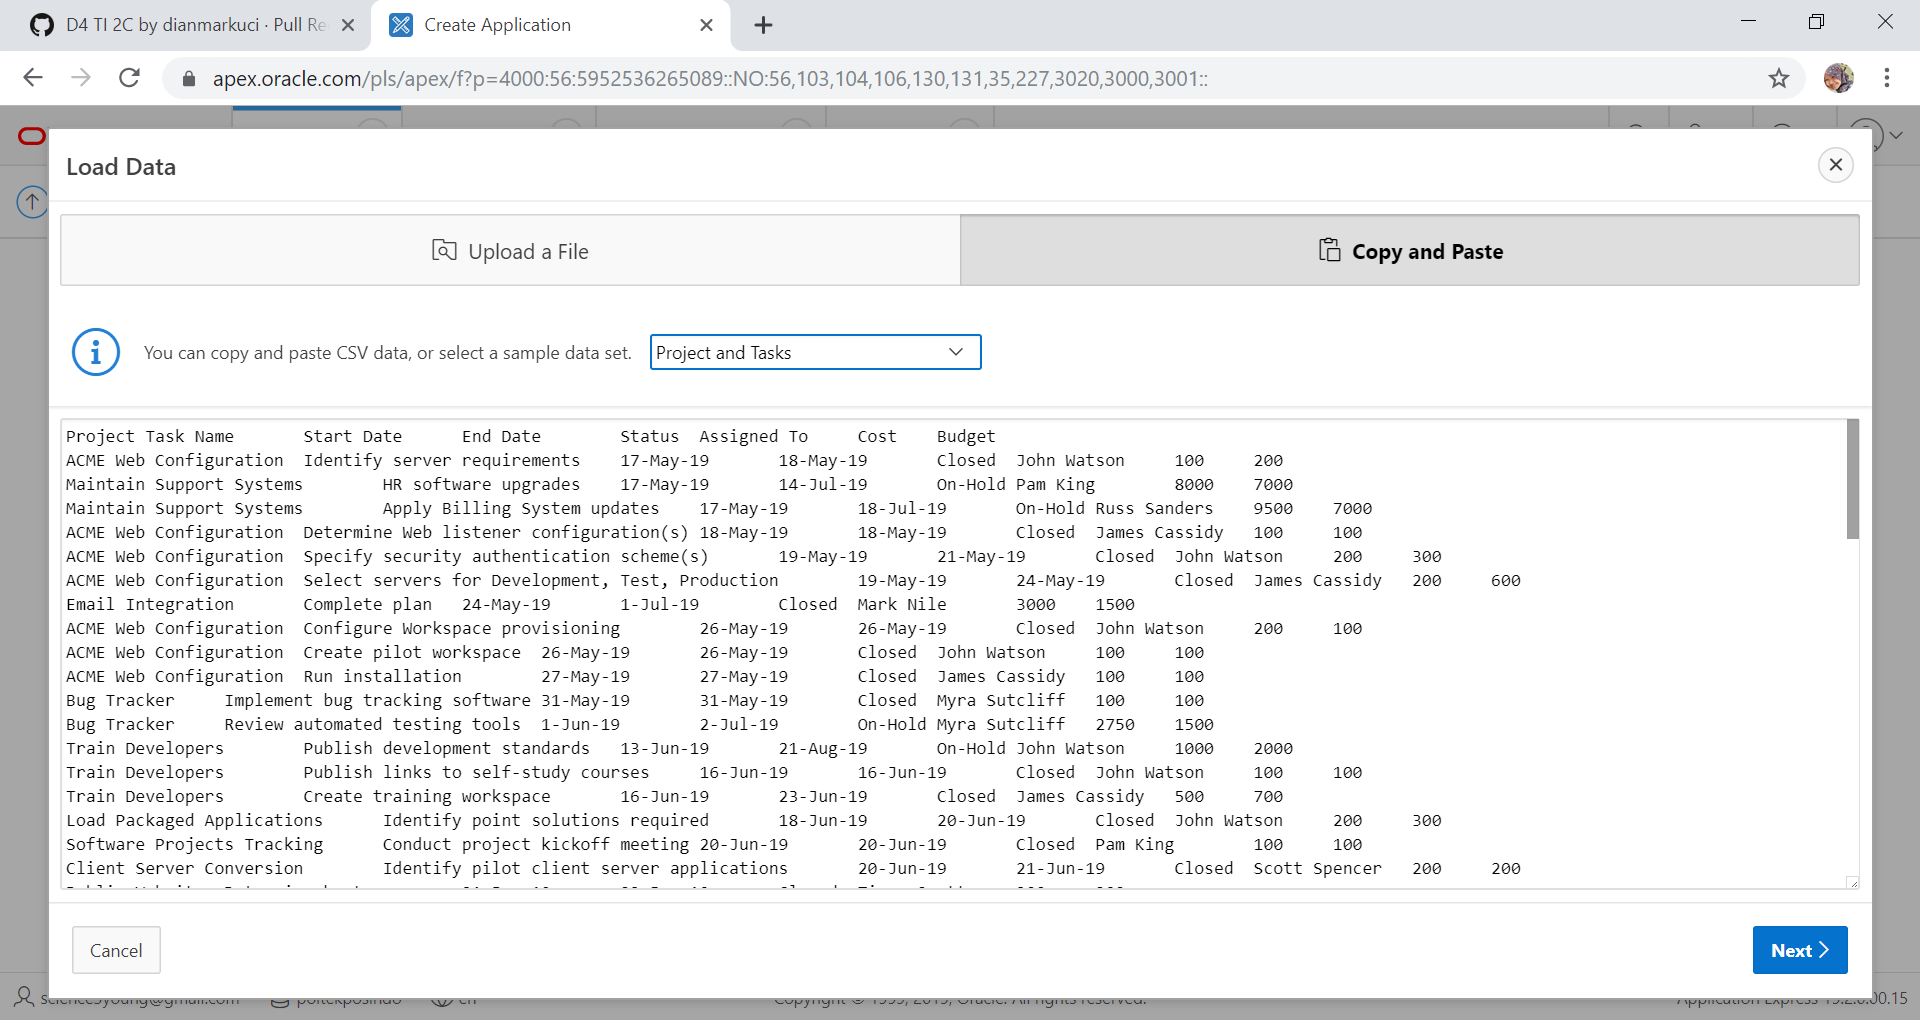
\includegraphics[scale=0.5]{figures/7.png}
        \caption{Membuat nama tabel dosen}
        \label{fig:my_label}
    \end{figure}
\newline
    \item Lalu configure dan klik load data , lalu klik X untuk keluar .
    \newline
    \item Kemudian membuat tabel Kuliah .
    \begin{figure}[!htbp]
        \centering
        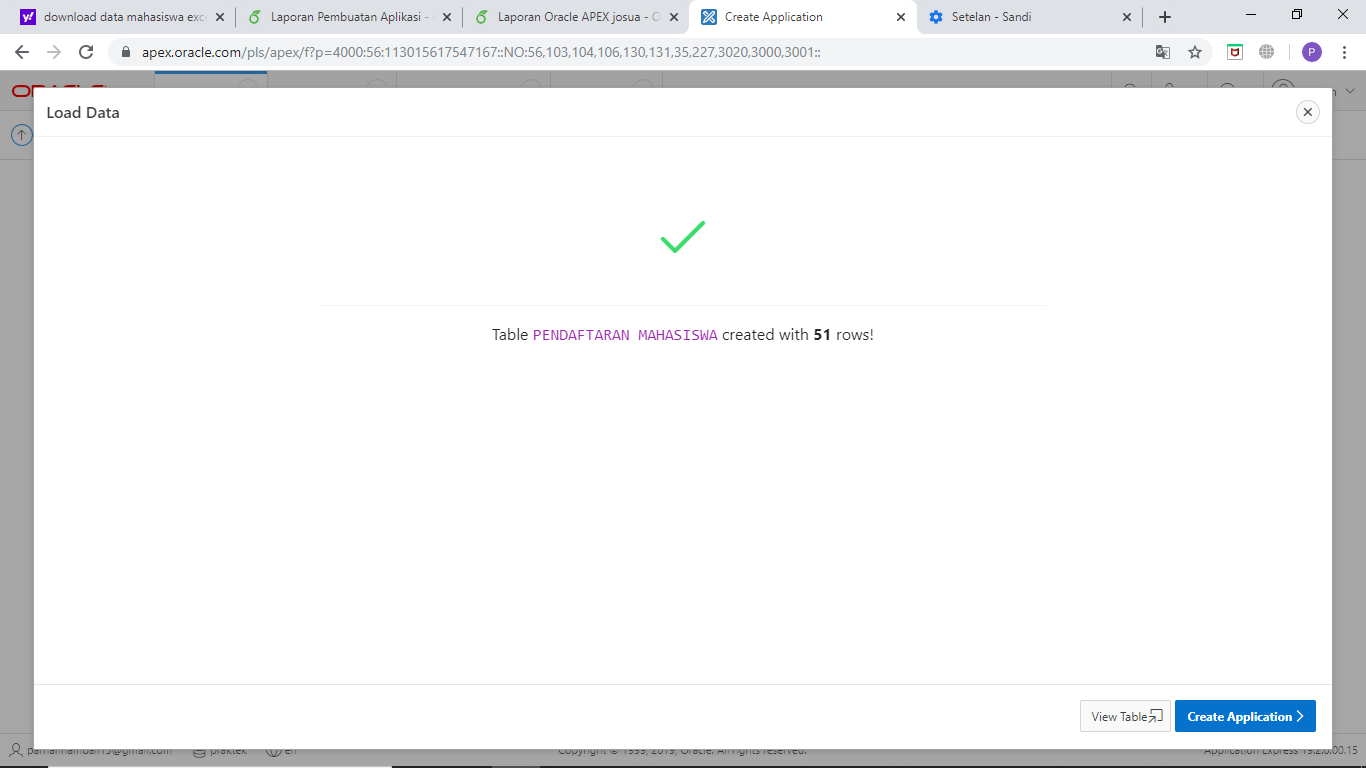
\includegraphics[scale=0.5]{figures/8.png}
        \caption{Membuat nama tabel kuliah}
        \label{fig:my_label}
    \end{figure}
    \newline
    \item Lakukan lagi perintah seperti diatas sampai semua tabel selesai dibuat . setelah tabel kuliah membuat tabel jadwal .
    \newline
    \begin{figure}[!htbp]
        \centering
        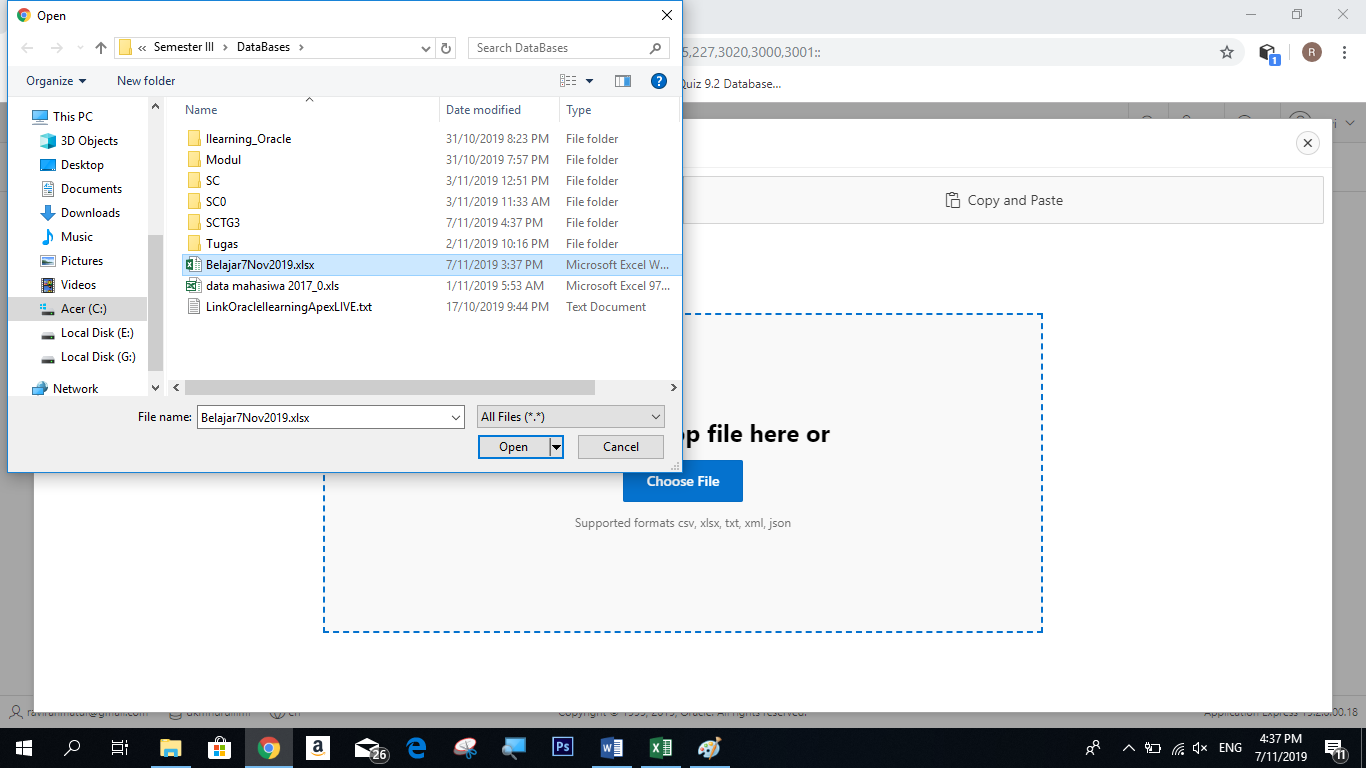
\includegraphics[scale=0.5]{figures/9.png}
        \caption{Membuat nama tabel jadwal}
        \label{fig:my_label}
    \end{figure}
    \newline
    \item Membuat tabel nilai . 
    \newline
    \begin{figure}[!htbp]
        \centering
        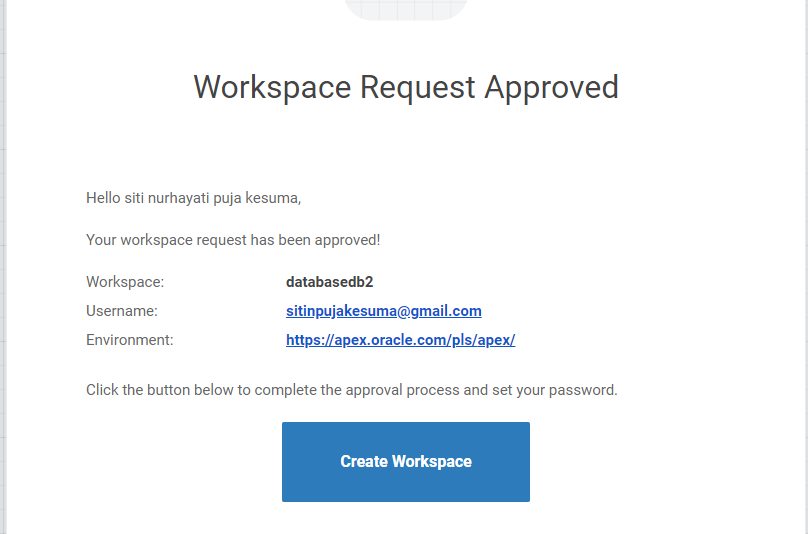
\includegraphics[scale=0.5]{figures/10.png}
        \caption{Mmebuat nama tabel nilai}
        \label{fig:my_label}
    \end{figure}
    \newline
    \item  Tampilan selanjutnya adalah create lalu hapus ID disetiap tabel .
\newline
\begin{figure}[!htbp]
    \centering
    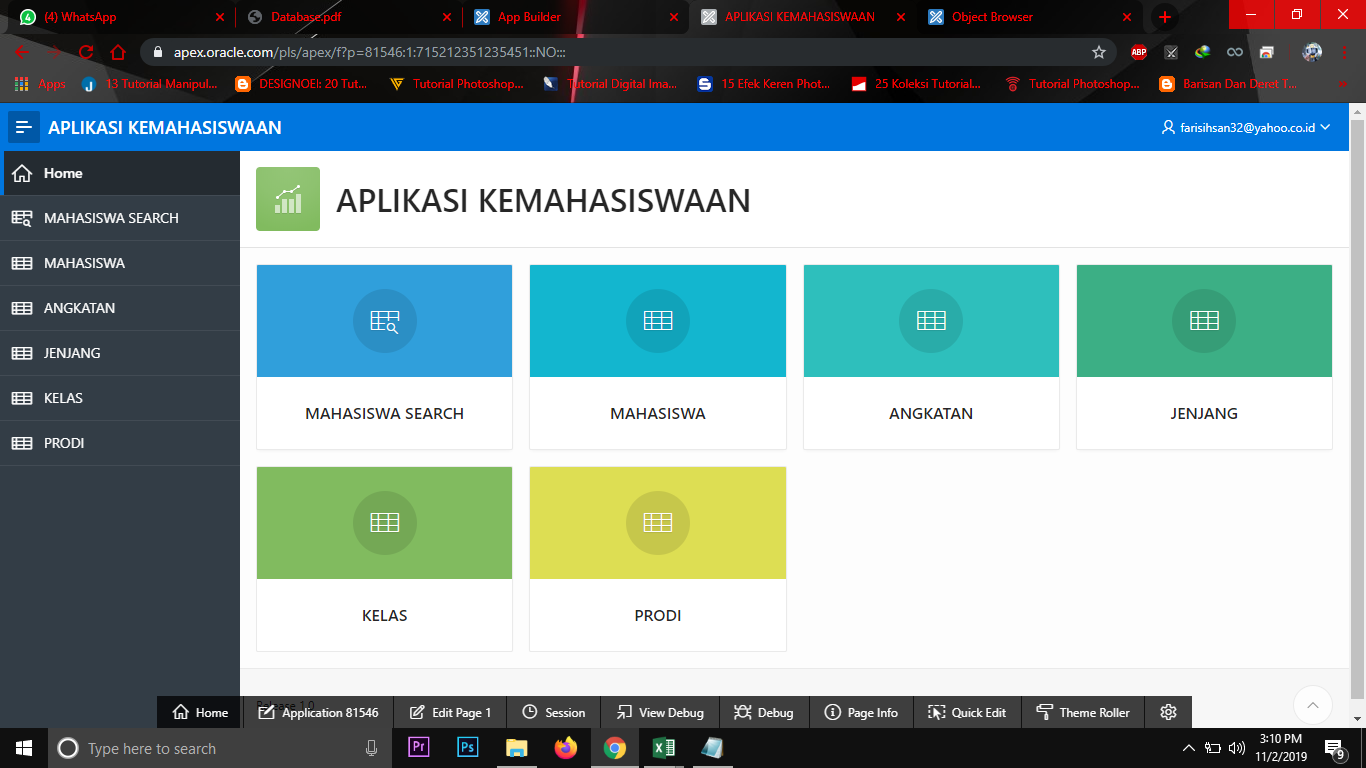
\includegraphics[scale=0.5]{figures/12.png}
    \caption{Menghapus ID}
    \label{fig:my_label}
\end{figure}
\newline
\item Lalu ubah setaip tabel ke primary dan foreign key , pertama kita ubah terlebih dahulu yang primary seperti Dosen , Mahasiswa dan kuliah sedangan jadwal dan nilai kita ubah ke foreign key .
\newline
\begin{figure}[!htbp]
    \centering
    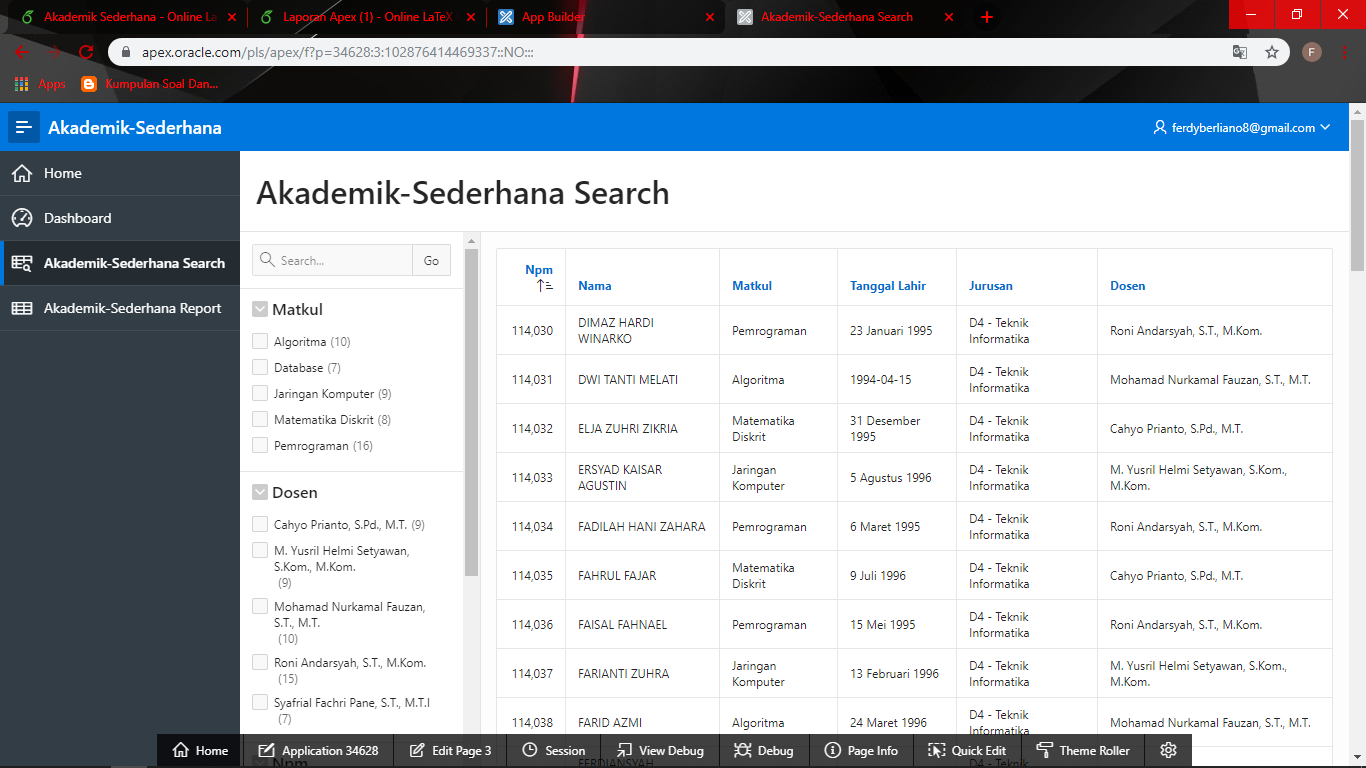
\includegraphics[scale=0.3]{figures/20.png}
    \caption{Mengubah tabel menjadi primary dan foreign key}
    \label{fig:my_label}
\end{figure}
\newline
\item Setelah itu kita buka app builder dan create .
\newline
\begin{figure}[!htbp]
    \centering
    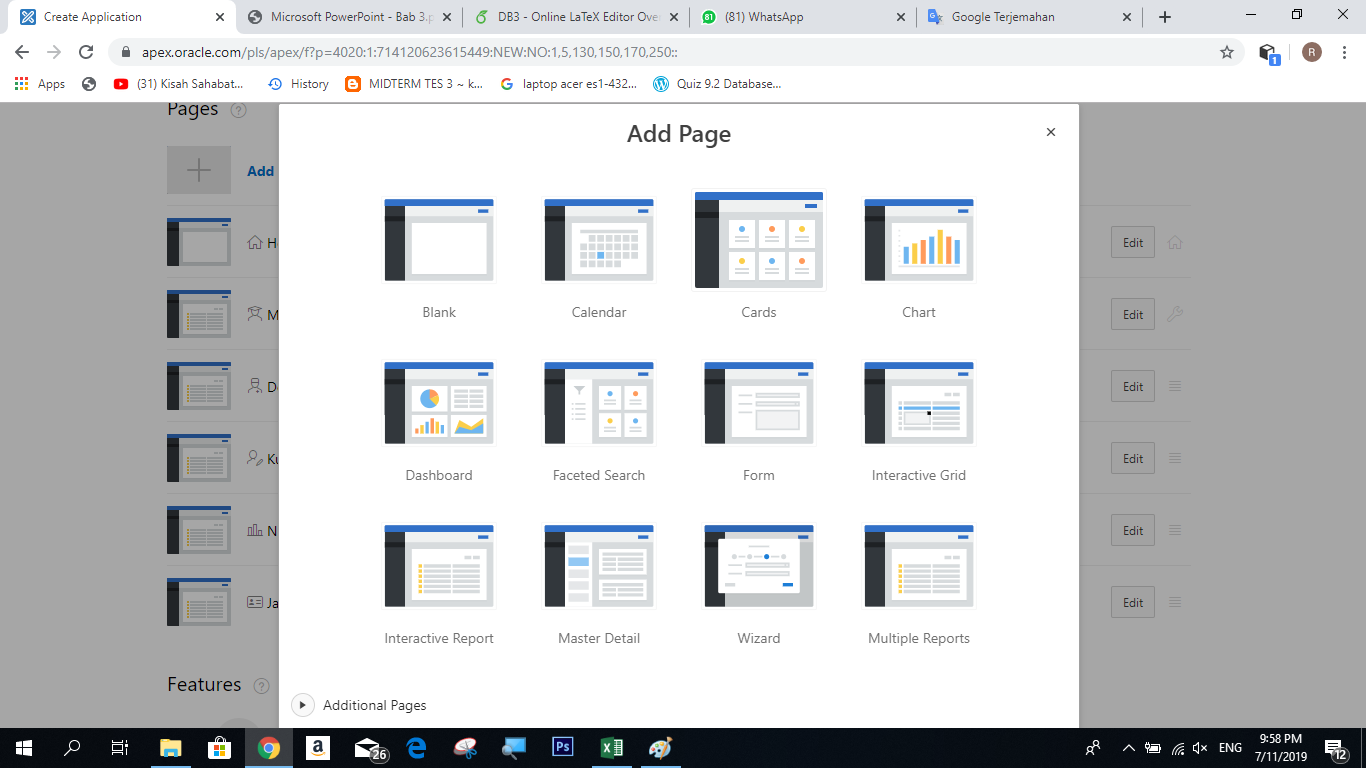
\includegraphics[scale=0.5]{figures/24.png}
    \caption{App Builder}
    \label{fig:my_label}
\end{figure}
\newline
\item Kemudian add page untuk memilih fitur apa saja yang mau digunakan . 
\newline
\begin{figure}[!htbp]
    \centering
    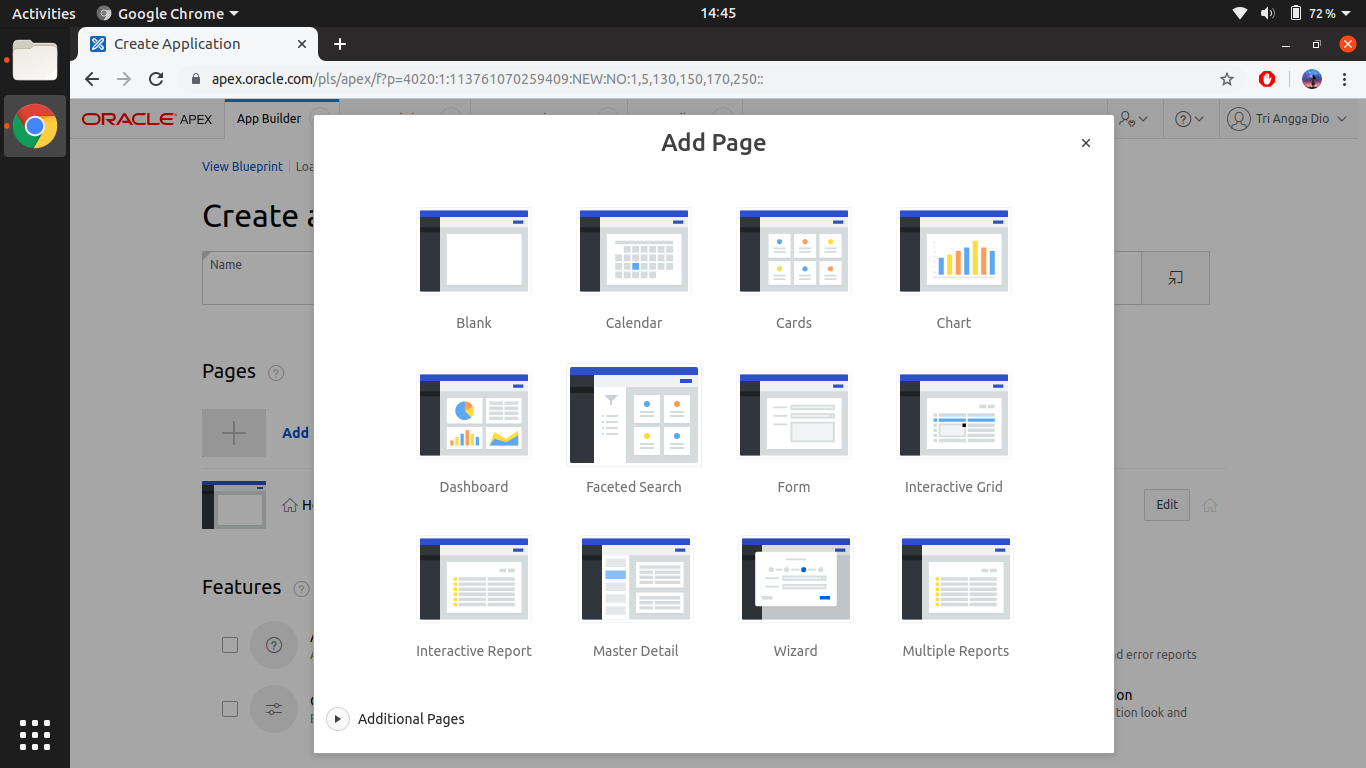
\includegraphics[scale=0.5]{figures/26.png}
    \caption{Add page}
    \label{fig:my_label}
\end{figure}
\newline
\item Setelah itu Create An application 
\newline
\begin{figure}[!htbp]
    \centering
    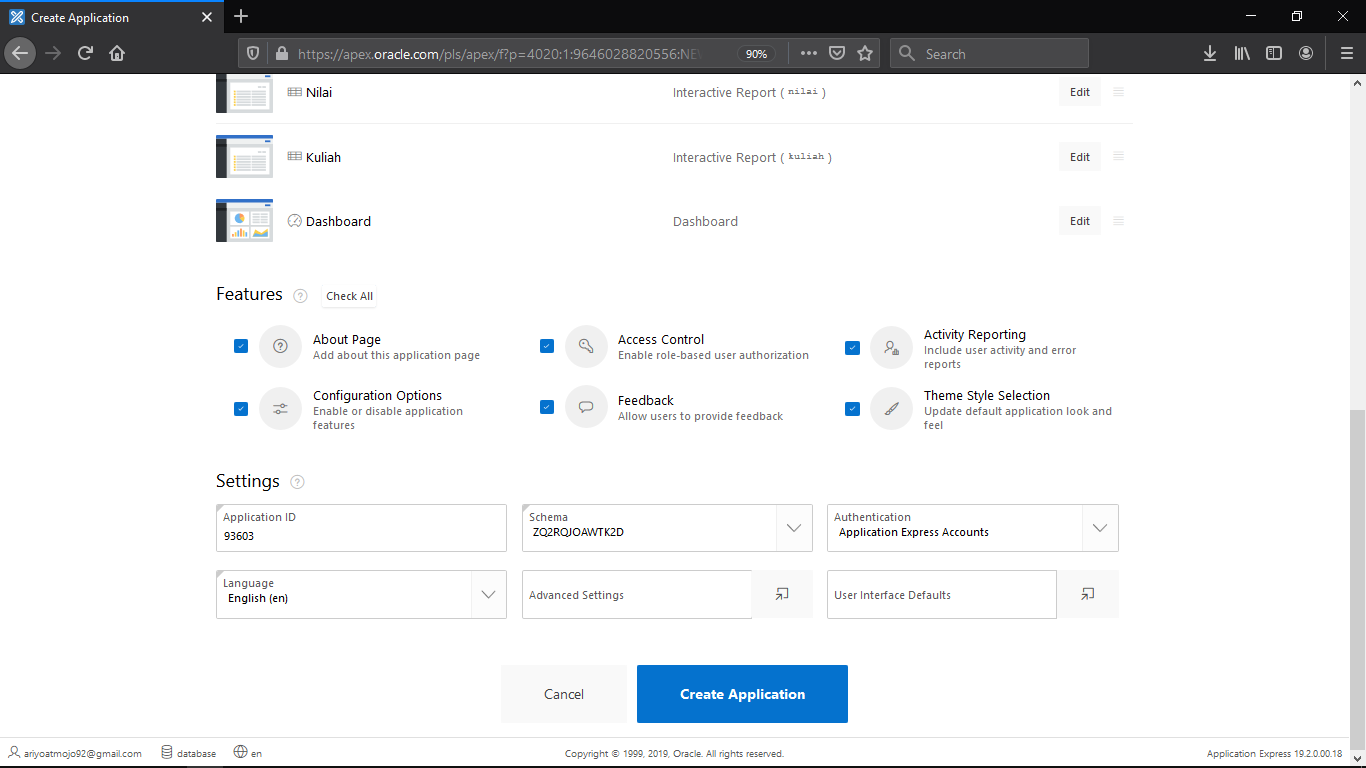
\includegraphics[scale=0.5]{figures/38.png}
    \caption{Create An Application}
    \label{fig:my_label}
\end{figure}
\newline
    \item  lalu klik check all
\newline
    \item  Maka selanjunya jalankan aplikasi dengan mengklik run application
\newline
\begin{figure}[!htbp]
    \centering
    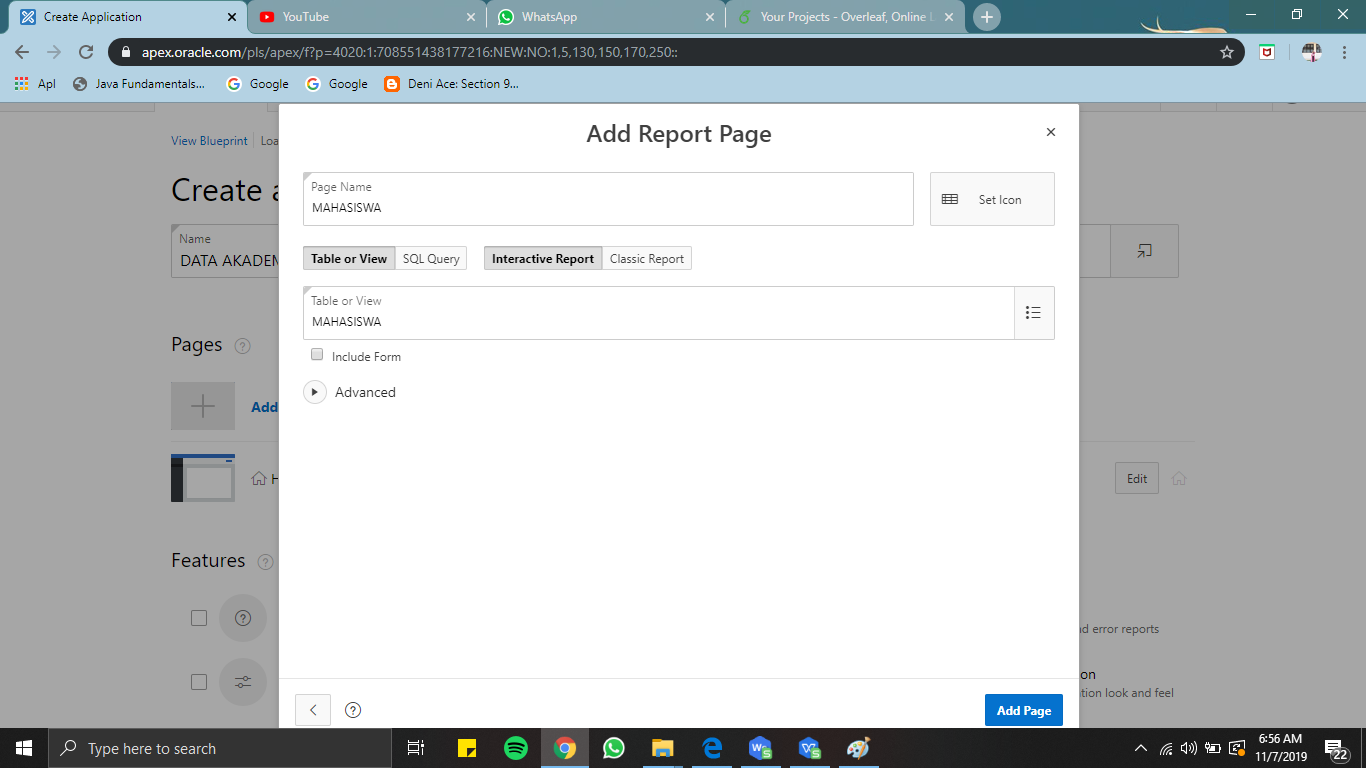
\includegraphics[scale=0.5]{figures/40.png}
    \caption{Run Application}
    \label{fig:my_label}
\end{figure}
\newline

\item Lalu masukkan email dan password untuk masuk ke aplikasi nya . 
\newline
\begin{figure}[!htbp]
    \centering
    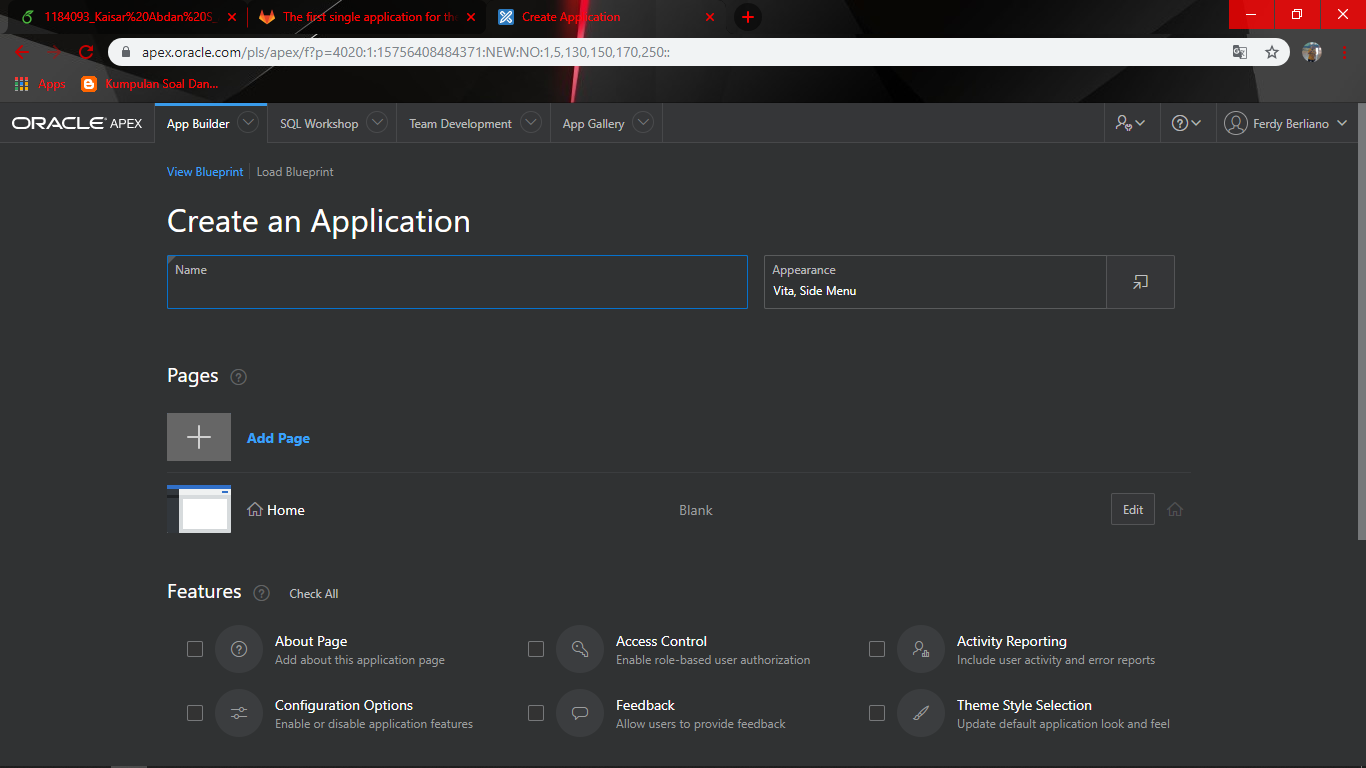
\includegraphics[scale=0.7]{figures/41.png}
    \caption{Sign in}
    \label{fig:my_label}
\end{figure}
\newline
    \item  Maka akan muncul aplikasi sistem sederhana akademik 
\newline
\begin{figure}[!htbp]
    \centering
    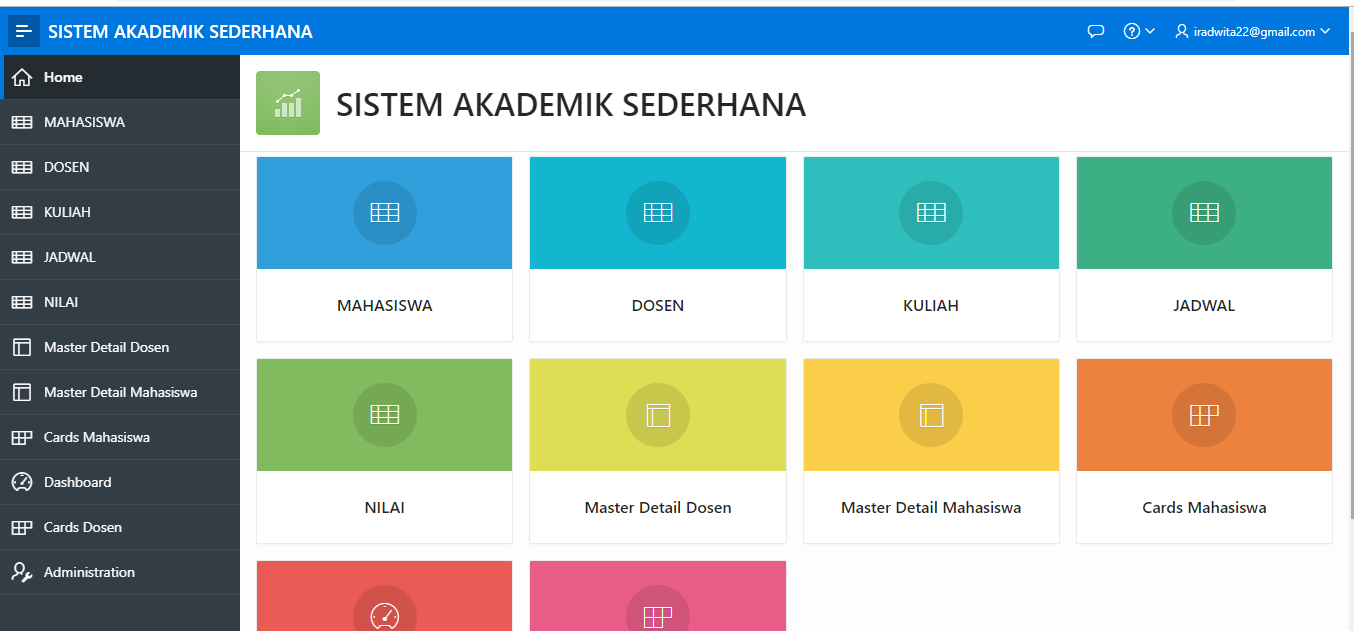
\includegraphics[scale=0.3]{figures/42.png}
    \caption{Aplikasi Sistem Akademik Sederhana}
    \label{fig:my_label}
\end{figure}
\newline
    \item  Aplikasi akademik selesai dibuat .
\end{enumerate}

link : https://apex.oracle.com/pls/apex/f?p=76816:LOGIN_DESKTOP:711761223598218:::::

Email : IRADWITA22@GMAIL.COM

Password :#Ira1234






\begin{enumerate}


\end{enumerate}
 
\chapter*{Link Oracle Express}
\section*{Data email password dan link oracle express} 


\item Email : jefriiimarbun@gmail.com
\item Password : jubilate300
\item https://apex.oracle.com/pls/apex/f?p=62374:1:20283547428623:::::

	
	
	
 
\chapter{Fungsi dan Kelas}
Tujuan pembelajaran pada pertemuan ketiga antara lain:
\begin{enumerate}
\item
Mengenal struktur fungsi di python dalam satu file dan cara pemanggilannya
\item
Mengerti cara membuat library fungsi dan melakukan import dan berbagai jenis import
\item
Mengerti struktur library kelas python dan cara pemakaiannya
\item
Mengatasi Error yang terjadi akibat pemakaian fungsi dan kelas
\item
Try Except
\end{enumerate}
Tugas dengan cara dikumpulkan dengan pull request ke github dengan menggunakan latex pada repo yang dibuat oleh asisten IRC. Kode program dipisah dalam folder src NPM.py yang berisi praktek dari masing-masing tugas file terpisah sesuai nomor yang kemudian dipanggil menggunakan input listing ke dalam file latex penjelasan atau nomor pengerjaan. Masing masing soal bernilai 5 dengan total nilai 100. Gunakan bahasa yang baku dan bebas plagiat dengan dibuktikan hasil scan plagiarisme. Serta hasil scrinsut dari komputer sendiri, dan kode hasil sendiri.

\section{Contoh Program}
\subsection{Fungsi}
Fungsi adalah satu blok program yang terdiri dari nama fungsi, input variabel dan variabel kembalian. Nama fungsi diawali dengan \textit{def} dan setelahnya tanda titik dua. Nama bisa sama dengan isi berbeda jika menggunakan huruf besar dan kecil atau sering disebut dengan \textit{case sensitive}. Input variabel bisa lebih dari satu dengan pemisah tanda koma. variabel kembalian pasti satu, bebas apakan itu jenis \textit{string}, \textit{integer}, \textit{list} atau \textit{dictionary}. Contoh dari fungsi sederhana bisa dilihat pada listing \ref{lst:fungsisederhana}. Dimana hasil akhir variabel c adalah 15.
\begin{lstlisting}[caption=Fungsi Sederhana,label={lst:fungsisederhana}]
def Penambahan(a,b):
	r = a + b
	return r
	
	
a=2
b=13
c = Penambahan(a,b)
\end{lstlisting}
sekarang kita pisah fungsi dengan pemakaian fungsi tersebut dalam file terpisah. Kita buat file bernama \textit{kalkulator.py} yang berisi semua fungsi penambahan, pengurangan, perkalian dan pembagian seperti terlihat pada listing \ref{lst:kalkulatorlib}. Sehingga satu file yang hanya berisi semua fungsi ini kita namakan \textit{paket} atau \textit{library}.
\begin{lstlisting}[caption=Library atau Paket kalkulator,label={lst:kalkulatorlib}]
def Penambahan(a,b):
	r = a + b
	return r
def Pengurangan(a,b):
	r = a - b
	return r
def Perkalian(a,b):
	r = a * b
	return r
def Pembagian(a,b):
	r = a / b
	return r
\end{lstlisting}
	Dan satu file yang memakai fungsi tersebut dengan nama file \textit{main.py}. Karena file kalkulator.py merupakan sebuah library maka kita panggil dulu dengan menggunakan perintah \textit{import}. Harus diingat file \textit{kalkulator.py} harus satu folder dengan \textit{main.py} yang berisi seperti listing\ref{lst:pakaikalkulator}.
\begin{lstlisting}[caption=Cara penggunaan library kalkulator,label={lst:pakaikalkulator}]
import kalkulator

a=100
b=50
hasil1=kalkulator.Penambahan(a,b)
hasil2=kalkulator.Pengurangan(a,b)
hasil3=kalkulator.Perkalian(a,b)
hasil4=kalkulator.Pembagian(a,b)
\end{lstlisting}
Maka kita bisa lihat hasilnya pada variabel hasil1, hasil2, hasil3, hasil4. Pada variabel exporer di spyder.

\subsection{Kelas}
Dasarnya dari kelas adalah pemrograman berbasis objek. Maka kita harus ingat, ada kelas ada objek ada atribut ada method. Fungsi kalkulator kita ubah menjadi kelas Ngitung.py menjadi seperti pada listing \ref{lst:kelasngitung}.
\begin{lstlisting}[caption=Kelas library kalkulator,label={lst:kelasngitung}]
class Ngitung:
  def __init__(self, a, b):
    self.a = a
    self.b = b
  def Penambahan(self):
    r = self.a + self.b
    return r
  def Pengurangan(self):
    r = self.a - self.b
    return r
  def Perkalian(self):
    r = self.a * self.b
    return r
  def Pembagian(self):
    r = self.a / self.b
    return r
\end{lstlisting}
Dana pada file main.py untuk menggunakan kelas maka bedanya adalah penambahan variabel yang menjadi objek instansiasi dari kelas seperti terlihat pada listing \ref{lst:instanngitung}.
\begin{lstlisting}[caption=Cara penggunaan kelas library kalkulator,label={lst:instanngitung}]
import ngitung

a=100
b=50

hitung = ngitung.Ngitung(a,b)

hasil1=hitung.Penambahan()
hasil2=hitung.Pengurangan()
hasil3=hitung.Perkalian()
hasil4=hitung.Pembagian()
\end{lstlisting}



\section{Pemahanan Teori}
Kerjakan soal berikut ini, masing masing bernilai 5. 
Praktek teori penunjang yang dikerjakan :
\begin{enumerate}
\item
Apa itu fungsi, inputan fingsi dan kembalian fungsi dengan contoh kode program lainnya.
\item
Apa itu paket dan cara pemanggilan paket atau library dengan contoh kode program lainnya.
\item
Jelaskan Apa itu kelas, apa itu objek, apa itu atribut, apa itu method dan contoh kode program lainnya masing-masing.
\item
Jelaskan cara pemanggikan library kelas dari instansiasi dan pemakaiannya dengan contoh program lainnya.
\item
Jelaskan dengan contoh pemakaian paket dengan perintah \textit{from kalkulator import Penambahan} disertai dengan contoh kode lainnya.
\item
Jelaskan dengan contoh kodenya, pemakaian paket fungsi apabila file library ada di dalam folder.
\item
Jelaskan dengan contoh kodenya, pemakaian paket kelas apabila file library ada di dalam folder.
\end{enumerate}

\section{Ketrampilan Pemrograman}
Kerjakan soal berikut ini, masing masing bernilai 5. Pada pertemuan sebelumnya tentang pembuatan program di python, sekarang cobalah untuk membuat nya dalam bentuk fungsi dan kelas dengan ketentuan:
\begin{enumerate}
\item
Buatlah fungsi dengan inputan variabel NPM, dan melakukan print luaran huruf yang dirangkai dari tanda bintang, pagar atau plus dari NPM kita.
Tanda bintang untuk NPM mod 3=0, tanda pagar untuk NPM mod 3 =1, tanda plus untuk NPM mod3=2.
Contoh Output : 
\begin{verbatim}
*****    *** ******     *****    ****
*******  *** ***  **    *** **  *****
***  ******* ******     ***  **** ***
***    ***** ***        ***       ***
***     **** ***        ***       ***
\end{verbatim}
NPM sesuai dengan nomor NPM nya.
\item
Buatlah fungsi dengan inputan variabel berupa NPM. kemudian dengan menggunakan perulangan mengeluarkan print output sebanyak dua dijit belakang NPM, 
contoh NPM : 113040087 maka akan ada output sebanyak 87 dengan tulisan `Hallo, 113040087 apa kabar?'
\begin{verbatim}
Output : 
Halo, 113040087 apa kabar? 
Halo, 113040087 apa kabar?
Halo, 113040087 apa kabar?
Halo, 113040087 apa kabar?
Halo, 113040087 apa kabar?
Halo, 113040087 apa kabar?
Halo, 113040087 apa kabar?
Halo, 113040087 apa kabar?
.....87 kali...
\end{verbatim}
\item
Buatlah fungsi dengan dengan input variabel string bernama \textbf{NPM} dan beri luaran output dengan perulangan berupa tiga karakter belakang dari NPM sebanyak penjumlahan tiga dijit tersebut. Penjumlahan dilakukan dengan menggunakan operator aritmatika dan fungsi int() atau str().
\begin{verbatim}
Output : Halo, Nama apa kabar? 
Halo, 087 apa kabar?
Halo, 087 apa kabar?
Halo, 087 apa kabar?
Halo, 087 apa kabar?
Halo, 087 apa kabar?
Halo, 087 apa kabar?
Halo, 087 apa kabar?
........15 kali(0+8+7).........
\end{verbatim}
\item
Buatlah fungsi hello word dengan input variabel string bernama \textbf{NPM} dan beri luaran output berupa digit ketiga dari belakang dari variabel NPM menggunakan akses langsung manipulasi string pada baris ketiga dari variabel NPM.
\begin{verbatim}
Input : 113040087
Output :
Halo, 0 apa kabar?
\end{verbatim}
\item

\label{digitvar2}
(wajib menggunakan perulangan dan atau kondisi) buat fungsi program dengan input variabel NPM dan melakukan print nomor npm satu persatu kebawah.
Contoh untuk NPM : 113040087 maka,
\begin{verbatim}
1
1
3
0
4
0
0
8
7
\end{verbatim}
\item
Buatlah fungsi dengan inputan variabel NPM, didalamnya melakukan penjumlahan dari seluruh dijit NPM tersebut, wajib menggunakan perulangan dan atau kondisi.
\item 
Buatlah fungsi dengan inputan variabel NPM, didalamnya melakukan melakukan perkalian dari seluruh dijit NPM tersebut, wajib menggunakan perulangan dan atau kondisi.
\item
Buatlah fungsi dengan inputan variabel NPM, Lakukan print NPM anda tapi hanya dijit genap saja. wajib menggunakan perulangan dan atau kondisi. Contoh jika NPM :113040087.
\begin{verbatim}
48
\end{verbatim}
\item
Buatlah fungsi dengan inputan variabel NPM, Lakukan print NPM anda tapi hanya dijit ganjil saja. wajib menggunakan perulangan dan atau kondisi. Contoh jika NPM :113040087.
\begin{verbatim}
1137
\end{verbatim}
\item 
Buatlah fungsi dengan inputan variabel NPM, Lakukan print NPM anda tapi hanya dijit yang termasuk bilangan prima saja. wajib menggunakan perulangan dan atau kondisi. Contoh jika NPM :113040087.
\begin{verbatim}
37
\end{verbatim}
\item
Buatlah satu library yang berisi fungsi-fungsi dari nomor diatas dengan nama file 3lib.py dan berikan contoh cara pemanggilannya pada file main.py.
\item
Buatlah satu library class dengan nama file kelas3lib.py yang merupakan modifikasi dari fungsi-fungsi nomor diatas dan berikan contoh cara pemanggilannya  pada file main.py.
\end{enumerate}


\section{Ketrampilan Penanganan Error}
Kerjakan soal berikut ini, masing masing bernilai 5. Bagian Penanganan error dari script python.
\begin{enumerate}
\item
Tuliskan peringatan error yang didapat dari mengerjakan praktek ketiga ini, dan jelaskan cara penanganan error tersebut.
dan Buatlah satu fungsi yang menggunakan gunakan try except untuk menanggulangi error yang kemungkinan akan terjadi.
\end{enumerate}

 
\chapter{PENYUSUNAN LAPORAN}
\section{Tujuan}
Untuk	 melaporkan	 jalannya	 pekerjan	 Proyek	 serta	 hasil	 yang	 diperoleh,	 mahasiswa	diwajibkan	menyusun	laporan	pekerjaan	Proyek.

\section{Ketentuan Penyusunan Laporan}
\subsection{Format Laporan}
Laporan	Proyek	hendaknya	berisi	:

\begin{enumerate}
\item \textbf{ Bagian Awal}
	\begin{itemize}
		\item Lembar	Muka	
		\item Lembar Pengesahan
		\item Surat	Pernyataan	Tidak	Melakukan	Plagiarisme
	 \item Abstrak	(dalam	Bahasa	Indonesia)
	 \item Abstract(dalam	Bahasa	Inggris)
	 \item Kata	Pengantar
	 \item Daftar	Isi	termasuk	:
 \begin{enumerate}[label=(\alph*)]
 
	\item Daftar	Gambar
	\item Daftar	Tabel
	\item Daftar	Simbol
	\item Daftar	Singkatan	
	\item Daftar	Lampiran
 \end{enumerate}
 \end{itemize}
 
\item \textbf{Bagian Isi}
 	\par \textbf{BAB	I PENDAHULUAN}
 	
 	\begin{enumerate} [label=1.\arabic*]
 	\item \textbf{ Latar	Belakang} \par 
Berisi	ulasan	ringkas	mengenai	keadaan/kondisi	yang	ada	dan	
kekurangan	 dari	 sistem	 yang	 diamati	 sehingga	 muncul	 topik	
yang	diambil.

\item \textbf{ Identifikasi	Masalah} \par 
Berisi	 berbagai	 masalah	 yang	 sudah	 dikenali	 dan	 	 akan diberikan	 solusinya	 melalui	 fungsi	 dari	 sistem/aplikasi/alat	yang	akan	dibuat.

\item \textbf{Tujuan} \par
Berisi	tujuan	untuk	apa	sistem/aplikasi/alat	itu	dibuat.

\item \textbf{ Ruang	Lingkup	} \par
Berisi	batasan-batasan	proyek	atau	cakupan	aplikasi	yang	akan	
dibangun.

\item \textbf{ Sistematika	Penulisan} \par
Menjelaskan	isi	yang	ada	di	laporan	proyek.\\
 
 	\end{enumerate}
 	
 \par \textbf{BAB II LANDASAN TEORI} \par 
 
 	Uraian	 \textbf{tentang	 teori yang	 mendukung} Objek	 PROYEK 2.	 \textbf{Harus	jelas	 sumber	 rujukannya	 dari	 mana}. Sumber	 yang	 baik	 adalah	jurnal	 ilmiah,	 artikel	 ilmiah,	 buku,	 dll.	 \textit{\textbf{Disarankan	 untuk	 tidak	mengambil	sumber	seperti	WebBlog,	Wikipedia,	dll.}} \\
 	
 	\par \textbf{BAB III ANALISIS DAN PERANCANGAN} \par 
 	\textit{\textbf{Analisis}} : \par 
 	Proses	 untuk	 menentukan	 bentuk	 dari	 kebutuhan	
sistem/aplikasi/alat	 baik	 berupa	 kebutuhan	 pada	 saat	membangun	
maupun	pada	saat	Implementasi.

	\textit{\textbf{Perancangan}}: \par 
	Penjelasan	 perancangan	 	 sistem/aplikasi/alat	 	 yang	 akan	 dibuat	terdiri	dari	perancangan	alir	program \textit{\textbf{(Flow	Chart)}}	, algoritma,	data,	maupun	perancangan	input/output	sistem/aplikasi/alat.		
 	
	
	\begin{enumerate} [label=3.\arabic*]
		\item Analisis
			\begin{enumerate} [label=3.1.\arabic*]
				\item Analisis	Sistem	yang	Sedang	Berjalan
					\begin{enumerate} [label=3.1.1.\arabic*]
						\item Analisis	Prosedur/ \textit{Flow	Map} yang								  berjalan
						\item Analisis	Dokumen	yang digunakan
					\end{enumerate}
				\item Analisis	Sistem	yang	akan	Dibangun
					\begin{enumerate} [label=3.1.2.\arabic*]
						\item Analisis	Kebutuhan	Aplikasi
						\item Analisis	Kebutuhan	Perangkat	lunak									  dan	Perangkat Keras
					\end{enumerate}
			\end{enumerate}
			
			
		\item Perancangan \textit{\textbf{(Jika	menggunakan	procedural 					  atau DFD)}}
			\begin{enumerate} [label=3.2.\arabic*]
				\item \textit{Context	Diagram}
				\item \textit {Data	Flow	Diagram} (disertai	tabel									  spesifikasi	Proses)
				\item Kamus	Alir	Data \textit{(Data Dictionary)}
				\item 	Perancangan	 \textit{Database (Sesuaikan	Format							Penulisannya)}
					\begin{enumerate} [label=3.2.4.\arabic*]
						\item \textit{Conceptual	Data	Model}
						\item \textit{Physical	Data	Model}
						\item \textit{Kamus	Data	Tabel (Database)}	
					\end{enumerate}
				\item Struktur Menu
				\item Perancangan Antarmuka
			\end{enumerate}
			
	\end{enumerate}
			
			\begin{enumerate} [label=3.2]
				\item Perancangan \textit{\textbf{(Jika	menggunakan 							  	Object	Oriented UML)}}
			\end{enumerate}
				\begin{enumerate} [label=3.2.\arabic*]
				\item \textit{Use	Case	Diagram}
				\item \textit{Class	Diagram}
				\item \textit{Interaction	Diagram}
				\item \textit{Sequence	Diagram}
				\item \textit{Collaboration	Diagram}
				\item \textit{Activity	Diagram}
				\item \textit{Statechart	Diagram}
				\item \textit{Componen	Diagram}
				\item \textit{Deployment	Diagram}
				\item \textit{Objek	Diagram}
				\item Perancangan \textit{Database (Sesuaikan	Format							  Penulisannya)}
						\begin{enumerate}[label=(\alph*)]
							\item \textit{Conceptual Data Model	(CDM)}
							\item \textit{Physical	Data Model (PDM)}
						\end{enumerate}
				\item Struktur	Menu
				\item Perancangan	Antarmuka
				\end{enumerate} 
				
	\par \textbf{BAB IV IMPLEMENTASI DAN PENGUJIAN} \par 
	\textbf{Implementasi} : \par 
	adalah	sistem/aplikasi/alat	yang	dibuat	dengan	merinci	komponenkomponen	 pendukung	 berupa	 program,	 Lingkungan	 Implementasi, Tampilan	Antarmuka,	Petunjuk	Pemakaian,	Petunjuk	Instalasi.
	
	\textbf{Pengujian} : \par 
	Adalah	 Cara	 untuk	 mengetahui	 apakah	 sistem/aplikasi/alat	 yang dibuat	sesuai	dengan	rancangan	dan	menuliskan	hasil	ujinya.
\textit{Jika	 anda	 membuat	 analisis	 sistem/aplikasi,	 maka	 harus	 seperti berikut:}
	
	\begin{enumerate} [label=4.\arabic*]
		\item Lingkungan	Implementasi \par 	
		Berisi	 perangkat	 lunak	 dan	 perangkat	 keras	 apa	 saja yang	digunakan	 sewaktu	 perancangan	 aplikasi	 berupa	 sistem	operasi,	database,	prosesor,	memory,	space	harddisk	dan	lain-lain	sesuai	dengan	kebutuhan serta	perangkat	pendukungnya.
		
		\item Pembahasan	Hasil	Implementasi \par 
		Berisi	 uraian	 hasil	 implementasi	 sistem	 yang	 disesuaikan	dengan	 tujuan	 pembuatan	 sistem.	 Jelaskan bahwa	 masalah	 yang	teridentifikasi	 pada	 identifikasi	 masalah yang berada	 di	 bab	 1	 telah	terseleseaikan, dan	 tujuan	 dari	 pelaksanaan	 proyek	telah tercapai. Penjelasan	dibantu	dengan	Tampilan	Antarmuka	aplikasi.
		
		\item Pengujian	dan	hasil	Pengujian \par 
		Berisi	identifikasi	 pengujian,	 rencana	 pengujian,	 deskripsi dan hasil	uji.	Metoda	yang	digunakan	misalnya \textit{white	box testing} dan \textit{	black	box	testing}
		
	\end{enumerate}	 
	
	
	
	\par \textbf{BAB V KESIMPULAN	DAN	SARAN} \par 
	
	\begin{enumerate} [label=5.\arabic*]
		\item \textbf{Kesimpulan} : \par 
				berisi	pencapaian	tujuan	dari	sistem/aplikasi/alat	                yang	dibuat.
		\item \textbf{Saran} : \par 
				berisi	hal-hal	atau	tujuan	dari	pembuatan	sistem/aplikasi/alat	yang dirasa	belum	sempurna	atau	 tidak	 tercapai.	Saran	juga	bisa	berupa	kondisi	 implementasi	 yang	 optimal	 bagi	 sistem/aplikasi/alat	 yang dibuat.
	\end{enumerate}
			
			
\item Bagian Akhir
 \begin{itemize}
 	\item Daftar	Pustaka		(Lampiran	8)
 	\item Lampiran
 	\item Tabel-tabel
 \end{itemize} 
 		 	
\end{enumerate}

\section{Ukuran	Kertas	dan	Ukuran	Huruf}

\begin{itemize}
	\item Penulisan	 dan	 ejaan	 menggunakan	 ketentuan	 bahasa	 Indonesia	 yang	 baik	 dan	
benar;
	\item Penulisan	diketik	dengan	komputer,	dengan	ketentuan	:
		\begin{enumerate}
			\item Jarak	1,5 spasi ;
			\item Lebar	sembir	kiri	4	cm ;
			\item Lebar	sembir	kanan	2,5	cm ;
			\item Lebar	sembir	atas	3	cm ;
			\item Lebar	sembir	bawah	3	cm ;
			\item Ukuran	Font	adalah	\textit{Times	New	Roman} 12	Kecuali	untuk	judul	bab	menggunakan	\textit{Times New Roman} dengan	ukuran	14.
		\end{enumerate}
		
	\item Ukuran	buku	adalah	A4	(21	x	29,7	Cm),	dengan	berat	kertas	80	gram;
	
	\item Sampul	depan	adalah	mika/softcover mika,	dengan	ketentuan	seperti	ini	:
		\begin{enumerate}
			\item Proposal	Proyek   \qquad \qquad \enspace : Mika Transparan .
			\item Buku Laporan Proyek \qquad : \textit{Softcover} Merah Omega 17.
		\end{enumerate}
		
		
\section{Ketentuan	Khusus}
	\begin{enumerate}
		\item \textbf{Abstrak} : Jarak	 1	 spasi,	 maksimal	 1	 halaman,	 font	 12,	 italic,	 maksimum	 200	 kata.
Hanya	1	paragraf. Kata	kunci	minimal	5.

		\item Penomoran	 tabel	 dilakukan	 dengan	 menyebutkan	 nomor	 bab,	 diikuti	 nomor	 urut	tabelnya	pada	bab	tersebut,	misalnya	Tabel	3.7,	artinya	tabel	nomor 7	di	bab	3.	Judul	
tabel	 diletakkan	 di	 atas	 tabel,	 penulisannya	 dengan	 huruf	 kapital	 di	 awal	 kata.	 Bila	tabel	 lebih	 panjang	 dari	 halaman,	 maka	 sambungan	 tabel	 pada	 halaman	 berikutnya	
diberi	judul	dengan	tulisan	: \textbf{(Lanjutan)}
		\item Tulisan	di	dalam	tabel	Jarak	1 spasi,	ukuran	huruf kurang	atau	sama	dengan \textit{font} 10 ( $\leq \textit{font}  10$). 	Judul	tabel	disimpan diatas	table	tanpa	jarak	spasi.
		
		\item Penomoran	 gambar	 dilakukan	 dengan	menyebutkan	 nomor	 bab,	 diikuti	 nomor	 urut	gambarnya	pada	bab	tersebut,	misalnya		Gambar	2.5,	artinya	gambar	nomor	5	di	bab	
2.			 Judul	gambar	diletakkan	di	bawah	gambar,	penulisannya	dengan	huruf	kapital	di	awal	kata.

		\item Penomoran	 halaman	 dimulai	 dari	 nomor	 1	 untuk	 tiap	 bab	 atau	 lampiran,	 dengan	
ketentuan	sebagai	berikut:	\\
			Penomoran	 dari	 bab	 1	 sampai	 bab	 5	 dimulai	 dari	 halaman	 1	 sampai	 selanjutnya	sekuensial	tanpa	menggunakan	bab	contoh	;	pada	awal	bab	2,	jika	bab	1	sebanyak	10	halaman,	maka	bab	2	dimulai	dengan	halaman	11	dst. .
			
		\item Penomoran	 halaman	 judul,	 buku	 laporan,	 halaman	 	 persetujuan,	 Daftar	 Isi,	 Daftar	Tabel,	dan	Daftar		Gambar	menggunakan	i,		ii,		iii,	…..	(angka	romawi	kecil).
		
		\item Setelah	Buku	laporan	 ditandatangani	 oleh	 pembimbing	 dan	 penguji	 seminar/sidang,	
maka	harus	di	buatkan	Jurnal	dengan	jumlah	halaman	maksimum	6	halaman.

		\item \textit{Softcopy} dari	jurnal, \textit{software} dan	laporan	disimpan	dalam	sebuah	CD	dan	disertakan	
ke	dalam	laporan di	beri	judul	serta	penulis	di	label	CD	nya.

	\end{enumerate}
\end{itemize}

\section{Status	Buku}
\begin{enumerate}
	\item Status Buku \par 
		Buku	 yang	 memenuhi	 persyaratan	 untuk	 sidang Proyek	 adalah	 buku	 yang	 telah	
selesai	 100 \%.	 Penjilidan	 buku	 sebelum	 sidang menggunakan	 penjepit	 dan	 sampul	plastik	mika	warna	Transparan;

	\item Setelah	Sidang \par 
		Buku	 yang	 memenuhi	 persyaratan	 untuk	 keluarnya	 nilai	 adalah	 buku	 yang	 telah	selesai	 100 \%	 (telah	 diperbaiki,	 jika	 ada	 tugas	 perbaikan).Penjilidan	 	 buku	 setelah	sidang dan	 setelah	 melalui	 perbaikan	 adalah	 jilid	 punggung	 disertai	 halaman	pembatas	bab	warna	merah	seperti	pita	pembatas	warna	merah.	
		
\end{enumerate}

\section{Distribusi	Buku}
Jumlah	 salinan	 laporan	 Proyek	 untuk	 keperluan	 sidang Proyek	 adalah	 3	 \textit{copy},	 dengan	distribusi	sebagai	berikut	:

\begin{enumerate}
	\item Pembimbing/Ketua	Penguji \quad (1 copy)
	\item Anggota	Penguji \qquad \qquad \qquad(1 copy)
	\item Mahasiswa \qquad \qquad \qquad \enspace \quad \quad(1 copy)
\end{enumerate}

Jumlah	salinan	buku	laporan	Proyek		adalah	4	 (empat) \textit{	 copy},	dengan	distribusi	sebagai	berikut	:

\begin{table}[H]
\label{tab:my-table}
\begin{tabular}{lll}
1 & Pembimbing & (1 CD) \\ \\
2 & Perpustakaan	Politeknik	Pos	Indonesia & (1 Buku dan CD ) \\ \\
3 & Mahasiswa & (1 Buku) \\ \\
4 & \multicolumn{2}{l}{\begin{tabular}[c]{@{}l@{}}Prodi	(1	 CD yang	 berisi	 jurnal,	 aplikasi	 dan	 laporan) dan	 hardcopy	 jurnal	 1	 buah	\\ tanpa	di	jilid.\end{tabular}}
\end{tabular}
\end{table}
 
\chapter{Komunikasi Perangkat Keras}

Tujuan pembelajaran pada pertemuan kelima antara lain:
\begin{enumerate}
\item
Mengenal komunikasi data serial
\item
Mengerti cara memakai library PySerial
\item
Mengerti cara instalasi driver dan menemukan BaudRate dan Nomor Port
\item
Mengatasi Error yang terjadi akibat pemakaian library csv dan pandas
\item
Try Except
\end{enumerate}
Tugas dengan cara dikumpulkan dengan pull request ke github dengan menggunakan latex pada repo yang dibuat oleh asisten IRC. Kode program dipisah dalam folder src NPM.py yang berisi praktek dari masing-masing tugas file terpisah sesuai nomor yang kemudian dipanggil menggunakan input listing ke dalam file latex penjelasan atau nomor pengerjaan. Masing masing soal bernilai 5 dengan total nilai 100. Gunakan bahasa yang baku dan bebas plagiat dengan dibuktikan hasil scan plagiarisme. Serta hasil scrinsut dari komputer sendiri, dan kode hasil sendiri. Pengerjaan menggunakan latex dan harus menyertakan file pdf hasil compile pdflatex, jika tidak diskon 50\%.


\section{Pemahaman Teori}
Kerjakan soal berikut ini, masing masing bernilai 5. Untuk hari pertama.
Praktek teori penunjang yang dikerjakan dengan deadline rabu jam 4 pagi:
\begin{enumerate}
\item
Apa itu fungsi device manager di windows dan folder /dev di linux
\item
Jelaskan langkah-langkah instalasi driver dari arduino
\item
Jelaskan bagaimana cara membaca baudrate dan port dari komputer yang sudah terinstall driver
\item
Jelaskan sejarah library pyserial
\item
Jelaskan fungsi-fungsi apa saja yang dipakai dari library pyserial
\item
Jelaskan kenapa butuh perulangan dalam tidak butuh perulangan dalam membaca serial
\item
Jelaskan bagaimana cara membuat fungsi yang mengunakan pyserial
\end{enumerate}

\section{Ketrampilan Pemrograman}
Kerjakan soal berikut ini, masing masing bernilai 10 untuk hari kamis jam 4 pagi. Soalnya adalah:

\begin{enumerate}
\item
Buatlah fungsi (file terpisah/library dengan nama NPM\_realtime.py) untuk mendapatkan data langsung dari arduino
\item
Buatlah fungsi (file terpisah/library dengan nama NPM\_save.py) untuk mendapatkan data langsung dari arduino dengan looping
\item
Buatlah fungsi (file terpisah/library dengan nama NPM\_realtime.py) untuk mendapatkan data dari arduino dan langsung ditulis kedalam file csv
\item
Buatlah fungsi (file terpisah/library dengan nama NPM\_csv.py) untuk membaca file csv hasil arduino dan mengembalikan ke fungsi
\end{enumerate}




\section{Ketrampilan Penanganan Error}
Kerjakan soal berikut ini, masing masing bernilai 5(hari kedua). Bagian Penanganan error dari script python.
\begin{enumerate}
\item
Tuliskan peringatan error yang didapat dari mengerjakan praktek ketiga ini, dan jelaskan cara penanganan error tersebut.
dan Buatlah satu fungsi yang menggunakan gunakan try except untuk menanggulangi error tersebut.
\end{enumerate}



\section{Presentasi Tugas}
Pada pertemuan ini, diadakan dua penilaiain yaitu penilaian untuk tugas mingguan seperti sebelumnya dengan nilai maksimal 100. Kemudian dalam satu minggu kedepan maksimal sebelum waktu mata kuliah pemrograman 3. Ada presentasi kematerian dengan nilai presentasi yang terpisah masing-masing 100. Jadi ada tiga komponen penilaiain pada pertemuan ini yaitu :
\begin{enumerate}
	\item tugas minggu hari ini dan besok (maks 100). pada chapter ini
	\item presentasi pyserial (maks 100). Mempraktekkan kode python dan menjelaskan cara kerjanya.
\end{enumerate}
Waktu presentasi pada jam kerja di IRC. Kriteria penilaian presentasi sangat sederhana, presenter akan ditanyai 20(10 pertanyaan program, 10 pertanyaan teori) pertanyaan tentang pemahamannya menggunakan python untuk kecerdasan buatan. jika presenter tidak bisa menjawab satu pertanyaan asisten maka nilai nol. Jika semua pertanyaan bisa dijawab maka nilai 100. Presentasi bisa diulang apabila gagal, sampai bisa mendapatkan nilai 100 dalam waktu satu minggu kedepan.




 
\chapter{Matplotlib}

Tujuan pembelajaran pada pertemuan kelima antara lain:
\begin{enumerate}
\item
Mengenal plot di python
\item
Mengerti cara memakai library Matplotlib
\item
Mengerti cara memplot berbagai macam jenis plot
\item
Mengatasi Error yang terjadi akibat pemakaian matplotlib
\item
Try Except
\end{enumerate}
Tugas dengan cara dikumpulkan dengan pull request ke github dengan menggunakan latex pada repo yang dibuat oleh asisten IRC. Kode program dipisah dalam folder src NPM.py yang berisi praktek dari masing-masing tugas file terpisah sesuai nomor yang kemudian dipanggil menggunakan input listing ke dalam file latex penjelasan atau nomor pengerjaan. Masing masing soal bernilai 5 dengan total nilai 100. Gunakan bahasa yang baku dan bebas plagiat dengan dibuktikan hasil scan plagiarisme. Serta hasil scrinsut dari komputer sendiri, dan kode hasil sendiri. Pengerjaan menggunakan latex dan harus menyertakan file pdf hasil compile pdflatex, jika tidak diskon 50\%.


\section{Pemahaman Teori}
Kerjakan soal berikut ini, masing masing bernilai 5. Untuk hari pertama.
Praktek teori penunjang yang dikerjakan dengan deadline hari pertama jam 4 pagi:
\begin{enumerate}
\item
Apa itu fungsi library matplotlib
\item
Jelaskan langkah-langkah membuat sumbu X dan Y di matplotlib
\item
Jelaskan bagaimana perbedaan fungsi dan cara pakai untuk berbagai jenis(bar,histogram,scatter,line dll) jenis plot di matplotlib
\item
Jelaskan bagaimana cara menggunakan legend dan label serta kaitannya dengan fungsi tersebut
\item
Jelaskan apa fungsi dari subplot di matplotlib, dan bagaimana cara kerja dari fungsi subplot, sertakan ilustrasi dan gambar sendiri dan apa parameternya jika ingin menggambar plot dengan 9 subplot di dalamnya
\item
Sebutkan semua parameter color yang bisa digunakan (contoh: m,c,r,k,... dkk)
\item
Jelaskan bagaimana cara kerja dari fungsi hist, sertakan ilustrasi dan gambar sendiri
\item
Jelaskan lebih mendalam tentang parameter dari fungsi pie diantaranya labels, colors, startangle, shadow, explode, autopct
\end{enumerate}

\section{Ketrampilan Pemrograman}
Kerjakan soal berikut ini, masing masing bernilai 10 untuk hari kedua jam 4 pagi. Soalnya adalah:

\begin{enumerate}
\item
Buatlah librari fungsi (file terpisah/library dengan nama NPM\_bar.py) untuk plot dengan jumlah subplot adalah NPM mod 3 + 2
\item
Buatlah librari fungsi (file terpisah/library dengan nama NPM\_scatter.py) untuk plot dengan jumlah subplot NPM mod 3 + 2
\item
Buatlah librari fungsi (file terpisah/library dengan nama NPM\_pie.py) untuk plot dengan jumlah subplot NPM mod 3 + 2
\item
Buatlah librari fungsi (file terpisah/library dengan nama NPM\_plot.py) untuk plot dengan jumlah subplot NPM mod 3 + 2
\end{enumerate}




\section{Ketrampilan Penanganan Error}
Kerjakan soal berikut ini, masing masing bernilai 5(hari kedua). Bagian Penanganan error dari script python.
\begin{enumerate}
\item
Tuliskan peringatan error yang didapat dari mengerjakan praktek ketiga ini, dan jelaskan cara penanganan error tersebut.
dan Buatlah satu fungsi yang menggunakan gunakan try except untuk menanggulangi error tersebut.
\end{enumerate}



\section{Presentasi Tugas}
Pada pertemuan ini, diadakan dua penilaiain yaitu penilaian untuk tugas mingguan seperti sebelumnya dengan nilai maksimal 100. Kemudian dalam satu minggu kedepan maksimal sebelum waktu mata kuliah pemrograman 3. Ada presentasi kematerian dengan nilai presentasi yang terpisah masing-masing 100. Jadi ada tiga komponen penilaiain pada pertemuan ini yaitu :
\begin{enumerate}
	\item tugas minggu hari ini dan besok (maks 100). pada chapter ini
	\item presentasi matplotlib (maks 100). Mempraktekkan kode python dan menjelaskan cara kerjanya.
\end{enumerate}
Waktu presentasi pada jam kerja di IRC. Kriteria penilaian presentasi sangat sederhana, presenter akan ditanyai 20(10 pertanyaan program, 10 pertanyaan teori) pertanyaan tentang pemahamannya menggunakan python untuk kecerdasan buatan. jika presenter tidak bisa menjawab satu pertanyaan asisten maka nilai nol. Jika semua pertanyaan bisa dijawab maka nilai 100. Presentasi bisa diulang apabila gagal, sampai bisa mendapatkan nilai 100 dalam waktu satu minggu kedepan.




 

%now enable appendix numbering format and include any appendices
%\appendix
%\chapter{Form Penilaian Jurnal}

gambar \ref{form1} dan \ref{form2} merupakan contoh bagaimana reviewer menilai jurnal kita. 
\begin{figure}[ht]
      \centerline{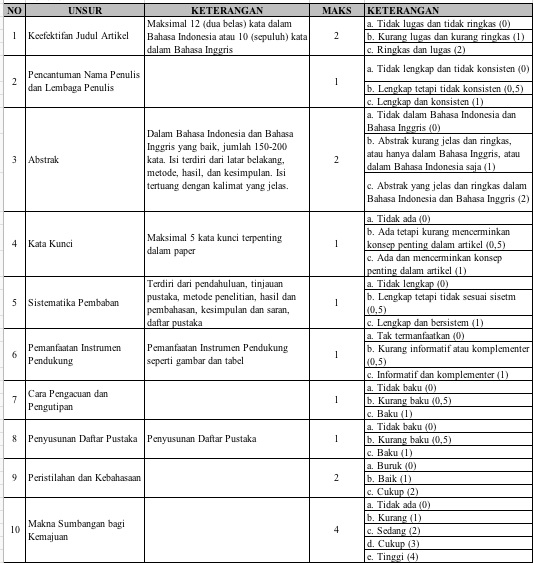
\includegraphics[width=1\textwidth]
      {figures/form1}}
      \caption{Form nilai bagian 1.}
      \label{form1}
      \end{figure}

	\begin{figure}[ht]
	      \centerline{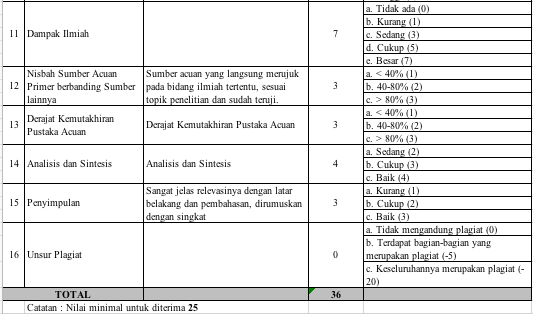
\includegraphics[width=1\textwidth]
	      {figures/form2}}
	      \caption{form nilai bagian 2.}
	      \label{form2}
	      \end{figure}

%\chapter{FAQ}

M : Kalo Intership II atau TA harus buat aplikasi ?
D : Ga harus buat aplikasi tapi harus ngoding

M : Pa saya bingung mau ngapain, saya juga bingung mau presentasi apa?
D : Makanya baca de, buka jurnal topik `ganteng' nah kamu baca dulu sehari 5 kali ya, 4 hari udah 20 tuh. Bingung itu tanda kurang wawasan alias kurang baca.

M : Pa saya sudah cari jurnal terindeks scopus tapi ga nemu.
D : Kamu punya mata de? coba dicolok dulu. Kamu udah lakuin apa aja? tolong di list laporkan ke grup Tingkat Akhir. Tinggal buka google scholar klik dari tahun 2014, cek nama jurnalnya di scimagojr.com beres.

M : Pa saya belum dapat tempat intership, jadi ga tau mau presentasi apa?
D : kamu kok ga nyambung, yang dipresentasikan itu yang kamu baca bukan yang akan kamu lakukan.

M : Pa ini jurnal harus yang terindex scopus ga bisa yang lain ?
D : Index scopus menandakan artikel tersebut dalam standar semantik yang mudah dipahami dan dibaca serta bukan artikel asal jadi. Jika diluar scopus biasanya lebih sukar untuk dibaca dan dipahami karena tidak adanya proses review yang baik dan benar terhadap artikel.

M : Pa saya tidak mengerti
D : Coba lihat standar alasan

M : Pa saya bingung
D : Coba lihat standar alasan

M : Pa saya sibuk
D : Mbahmu....

M : Pa saya ganteng
D : Ndasmu....

M : Pa saya kece
D : wes karepmu lah....


Biasanya anda memiliki alasan tertentu jika menghadapi kendala saat proses bimbingan, disini saya akan melakukan standar alasan agar persepsi yang diterima sama dan tidak salah kaprah. Penggunaan kata alasan tersebut antara lain :

1. Tidak Mengerti : anda boleh menggunakan alasan ini jika anda sudah melakukan tahapan membaca dan meresumekan 15 jurnal. Sudah mencoba dan mempraktekkan teorinya dengan mencari di youtube dan google minimal 6 jam sehari selama 3 hari berturut-turut.

2. Bingung : anda boleh mengatakan alasan bingung setelah maksimal dalam berusaha menyelesaikan tugas bimbingan dari dosen(sudah dilakukan semua). Anda belum bisa mengatakan alasan bingung jika anda masih belum menyelesaikan tugas bimbingan dan poin nomor 1 diatas. Setelah anda menyelesaikan tugas bimbingan secara maksimal dan tahap 1 poin diatas, tapi anda masih tetap bingung maka anda boleh memakai alasan ini.

%next line adds the Bibliography to the contents page
\addcontentsline{toc}{chapter}{Daftar Pustaka}
%uncomment next line to change bibliography name to references
%\renewcommand{\bibname}{References}
\bibliography{references}        %use a bibtex bibliography file refs.bib
\bibliographystyle{plain}  %use the plain bibliography style

\end{document}

